\section{Avoiding the Hands of the Sophists}

\begin{quotex}
When I had an inclination to philosophy, I did not fall into the hands of any sophist. \flright{\textsc{Marcus Aurelius}, \textit{Meditations}}

\end{quotex}

\begin{wrapfigure}{rt}{.3\textwidth}
 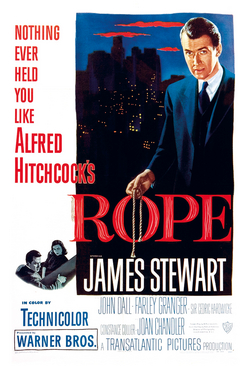
\includegraphics[scale=1.5]{a20130117AvoidingtheHandsoftheSophists-img001.jpg} 
\end{wrapfigure}

My son, who has been reading Meditations, asked me last night what a sophist is. I explained to him that a philosopher is a lover of wisdom while a sophist is a lover of his own words as well as the applause of other men. The sophist is paid for his opinions and will use any rhetorical device to make his case apart from considerations of facts or logic. I pointed out that we are awash with sophists today, all over television and radio; these talking heads are paid quite well to promote a certain point of view. Don't get me wrong, I am not simply saying they are necessarily cynical or hypocritical; they are still sophists even if they sincerely believe what they say. The next tier, those who provide the fodder for the more successful sophists, are apparently under the impression that every wandering influence that enters their head as a thought, is somehow worth repeating.

The first investigation of the philosopher when faced with a thought is to relate it to the transcendentals. Is it:

\begin{itemize}
\item True or false 
\item Good or bad 
\item Beautiful or ugly, or noble or vulgar 
\end{itemize}
The opinion mongers approach the thought in a different way. They ask instead

\begin{itemize}
\item Does it make me feel good or bad 
\item Does it improve my self-image 
\item Does it bring me esteem or cement the ``we" feeling of my group 
\end{itemize}
The more alert sophists boast of knowing all the philosophers. However, they do not know them in depth, i.e., in their principles, but rather they arrange them in easy to remember categories, just as my mother used to arrange Hummel figurines on shelves. They are easily recognizable since they sound like a professor leading a survey class at university. They will synopsize a great thinker or some long historical movement in a short sentence with a few adjectives.

\paragraph{Conversion}
Since the sophist knows so many systems, his mind is flighty, converting from one to another on a whim. These horizontal conversions are meant to bring on good feelings from an artificial high. Although partisans of various groups make use of them, they are pointless here. There are simply too many and it is always formulaic. Whether a man is converted by the Doctrine of Awakening, the Book of Mormon, Mein Kampf, the Communist Manifest, or Richard Dawkins, the formula is the same: the claim to a sudden insight, the instant obliteration of all past points of view, and the urge to evangelize. H L Mencken granted a man one such conversion in his life, but more than that is too much and the man could not be trusted.

We are more interested in two related conversions, or really two aspects of the same conversion:

\begin{description}
\item[Intellectual Conversion ]

The conversion from seeing the world horizontally in terms of things and events to understanding it vertically, in terms of principles. 

\item[Moral Conversion ]

The conversion from acting from the motives of likes, dislikes, desires, pleasures, and emotions to developing the wisdom, courage, and prudence or skillful means to act in terms of principles. 

\end{description}
It must be emphasized that these conversions are not related to ``intellectuality" as currently and popularly conceived, nor even to literacy. My son, for example, has sound instincts but lacks the rhetorical skills to express them in the written word. Throughout history, initiates were often illiterate, but no less initiated for that reason. In many ways that was a boon, since literacy today makes it easier for a man to absorb the dominant propaganda.

\paragraph{The Abyss}
Because of the lack of a common mind and the ubiquity of media today, we are bombarded with opinions: those of the shopkeepers, Christians, cows, females, Englishmen, and democrats are indiscriminately mixed in with those of the warrior [Freidrich Nietzsche, \emph{Twilight of the Idols}]. Here, Nietzsche displays his confusion or incomprehension. Which group in that list has historically eschewed pleasure to embrace difficulties, hardships, and privations, even life itself in the case of the martyrs? What about the warriors \textbf{Constantine}, \textbf{Charlemagne}, \textbf{Charles Martel}, the Templars and so on, who delight in war? Or is it only war without purpose that counts?

Some months back, I heard a neo-pagan on the radio, practically in tears about some alleged pagan holocaust of a millennium ago, claiming numbers as high as 10 million. He should have dropped the number by a few million to gain more credibility. But what was he really objecting to, if not to being among those human beings sacrificed for some other man's cause? I'll leave it to the more enterprising readers to locate the source for these two paragraphs.

It is true about the democrats, those who are ignorant about human nature, and whose only desire is that everyone be as timid as they themselves. We see that today in the USA over the ``gun control debate"; they believe a new law by a minimally competent government will forever end murders. Perhaps they are even allied with the neo-Christians of today. But we know that a murderous heart is hidden in the heart of darkness of the human being, from the time of Cain and Abel.

Your homework is to watch \textbf{Alfred Hitchcock}'s film, The Rope, in the upcoming month. Two young men murder a classmate to prove their superiority as \emph{uebermenschen}. They justify this from conversations with their professor who proclaimed Nietzsche's philosophy to them. The professor was appalled when he found out; presumably he was a cow or a woman, or more likely an armchair warrior. Yet their real sin was not the murder, but their choice of victim, someone too weak to strike back.

\paragraph{More Preparation}
My son was confirmed years ago at the Cathedral in West Palm Beach soon after the new Bishop was installed, whose name I have forgotten, and may memory of it be blotted out forever. Within weeks, as we were watching the nightly news, we heard that the Bishop had confessed to pedophilia. I recall to this day, the look of shock and bewilderment on my son's face. His only comment was that he was happy that the bishop hadn't touched him, since an auxiliary had confirmed him.

He is reasonably holy, but he won't step inside a church any more often than he has to. I can't argue with him, since they are seldom places where young men can feel comfortable. It is too easily forgotten that there are different spiritual practices for the different callings in life: the priest, the warrior, the creator. I know I have promised the put forth the views of the Frankish bishops on this and that is forthcoming. But meanwhile, there is much spiritual preparation that a man in the world can still perform.

We have previously explained that the candidate for initiation must demonstrate fearlessness, freedom from lust, loyalty, and the ability to be silent (omertà). Don't even consider initiation until you are properly prepared. For example, my son has these qualities so I know I can trust my life in his hands; should I have told him to pray the rosary daily instead?

A man, for his preparation, can conquer his fear of the elements: fire, air, water, and earth. Overcoming such fears leads to self-knowledge and a concentrated mind. Those with a warrior cast of mind need to excel at a martial art or develop skill with weaponry. Time spent in this way is more beneficial than excessive, or obsessive, reading. If you don't regard these activities as spiritual, then make them so. Do them with the right attitude and full consciousness.

Those who practice an art or a craft can do their work skillfully and fairly. This is spiritual preparation for the third caste. They can learn techniques of concentration, control over their thoughts, and development of the will. I think I have made too much of traditional practices such as prayer and contemplation, which are the way for a select few, and not enough of these other things. Perhaps a series on the development of the will is in order.



\flrightit{Posted on 2013-01-17 by Cologero }

\begin{center}* * *\end{center}

\begin{footnotesize}\begin{sffamily}



\texttt{william zeitler on 2013-01-19 at 11:50 said: }

I agree that the range of spiritual practices is considerably larger than the standard `meditation', etc. There are plenty of `trees of spiritual practices'–I partlcularly liked this one.

\url{http://www.contemplativemind.org/practices/tree}

Martial arts is one I fell into almost by accident, and it has done more to smooth out the rough edges of my soul than almost anything else. Also, as a professional musician, I've realized that I can turn doing my scales into its own spiritual practice–being fully present, etc.


\end{sffamily}\end{footnotesize}
